\documentclass[tikz,border=12pt]{standalone}
\usepackage[T1]{fontenc}
\usepackage{mathpazo}
\usepackage{amsmath,amssymb}
\usetikzlibrary{arrows.meta, positioning, calc, fit, decorations.pathreplacing}
\usepackage{pgfplots}
\pgfplotsset{compat=1.18}

\definecolor{stblue}{HTML}{7B97AD}
\definecolor{rwgold}{HTML}{B8995E}
\definecolor{sage}{HTML}{7A9A7E}
\definecolor{dkbrown}{HTML}{3D3530}
\definecolor{wmgray}{HTML}{7B7067}
\definecolor{cream}{HTML}{F9F6F0}
\definecolor{border}{HTML}{D4C9B8}
\definecolor{terracotta}{HTML}{C47A6A}
\definecolor{lavender}{HTML}{907EA0}

\begin{document}
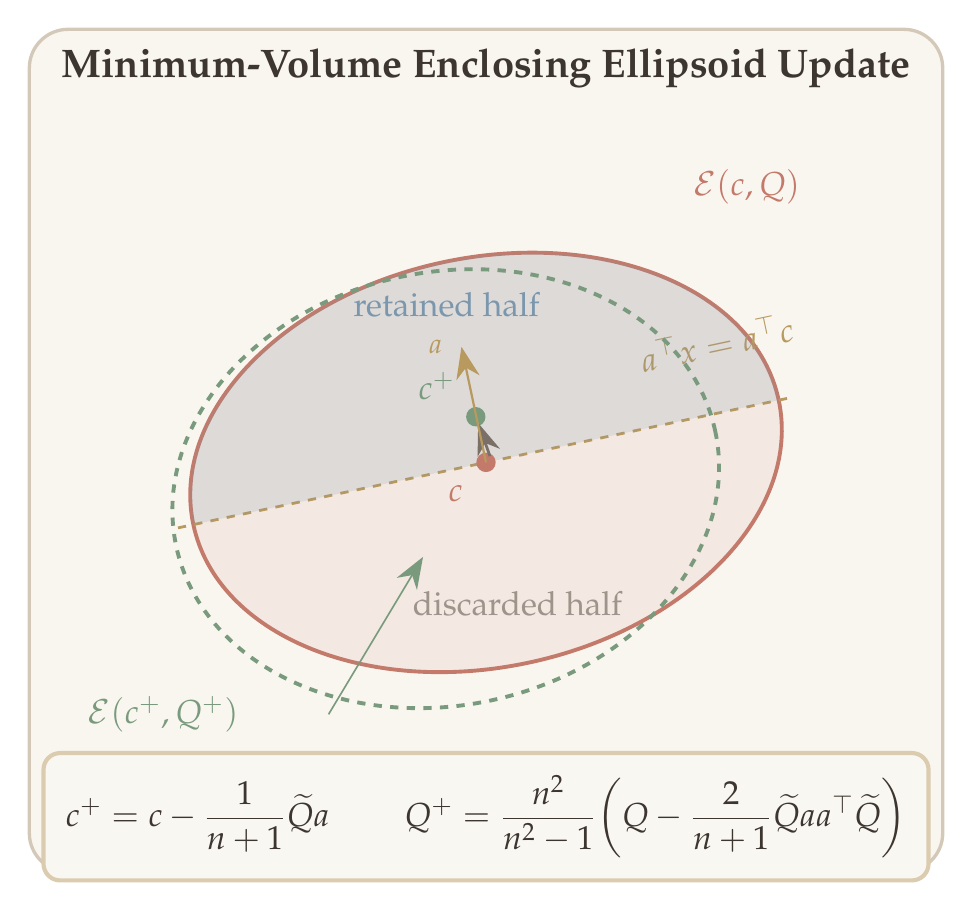
\begin{tikzpicture}[
    >={Stealth[length=4mm, width=3mm]},
    every node/.style={text=dkbrown},
    line width=1.5pt,
  ]

  % Background
  \fill[cream, rounded corners=14pt] (-5.8,-5.2) rectangle (5.8,5.5);
  \draw[border, line width=1.2pt, rounded corners=14pt] (-5.8,-5.2) rectangle (5.8,5.5);

  % Title
  \node[font=\Large\bfseries, text=dkbrown] at (0,5.0)
    {Minimum-Volume Enclosing Ellipsoid Update};

  % === Original ellipsoid (terracotta) ===
  \begin{scope}[rotate=12]
    \fill[terracotta, opacity=0.10] (0,0) ellipse (3.8cm and 2.6cm);
    \draw[terracotta, line width=1.4pt] (0,0) ellipse (3.8cm and 2.6cm);
  \end{scope}
  \node[font=\large\bfseries, text=terracotta, anchor=west] at (2.5,3.5)
    {$\mathcal{E}(c, Q)$};

  % === Cutting hyperplane (dashed rwgold) through center ===
  % Roughly perpendicular to the major axis direction (rotated 12 deg)
  % Cut normal direction: roughly (-sin12, cos12) ~ (-0.21, 0.98)
  % The line is perpendicular to this, so along (cos12, sin12)
  \draw[rwgold, line width=1.0pt, dashed]
    ({-4.0*cos(12)-0.0*sin(12)},{-4.0*sin(12)+0.0*cos(12)})
    -- ({4.0*cos(12)+0.0*sin(12)},{4.0*sin(12)-0.0*cos(12)});
  \node[font=\large\itshape, text=rwgold, anchor=south, rotate=12] at (3.0,1.2)
    {$a^\top x = a^\top c$};

  % === Shaded half-ellipsoid (the retained half, stblue) ===
  \begin{scope}
    \clip ({-4.0*cos(12)},{-4.0*sin(12)}) -- ({4.0*cos(12)},{4.0*sin(12)})
      -- ({4.0*cos(12)-4.0*sin(12)},{4.0*sin(12)+4.0*cos(12)})
      -- ({-4.0*cos(12)-4.0*sin(12)},{-4.0*sin(12)+4.0*cos(12)}) -- cycle;
    \begin{scope}[rotate=12]
      \fill[stblue, opacity=0.18] (0,0) ellipse (3.8cm and 2.6cm);
    \end{scope}
  \end{scope}
  \node[font=\large, text=stblue] at (-0.5,2.0) {retained half};

  % === New ellipsoid E(c^+, Q^+) (sage, dashed) ===
  \begin{scope}[rotate=12]
    \draw[sage, line width=1.4pt, dashed]
      (-0.57,-0.22) ellipse (3.5cm and 2.75cm);
  \end{scope}
  \node[font=\large\bfseries, text=sage, anchor=east] at (-3.0,-3.2)
    {$\mathcal{E}(c^+, Q^+)$};
  \draw[sage, line width=0.6pt, ->] (-2.0,-3.2) -- (-0.8,-1.2);

  % Center c (original)
  \fill[terracotta] (0,0) circle (3.5pt);
  \node[font=\large, text=terracotta, anchor=north east] at (-0.15,-0.15) {$c$};

  % Center c^+ (new, shifted into the retained half)
  % Shift along the cut normal direction: c^+ = c - (1/(n+1)) * Q * a_hat
  % Approximate: shift by (-0.21, 0.98) * ~0.6
  \fill[sage] (-0.13,0.58) circle (3.5pt);
  \node[font=\large, text=sage, anchor=south east] at (-0.25,0.65) {$c^+$};

  % Arrow from c to c^+
  \draw[wmgray, ->, line width=1.0pt] (0.05,0.08) -- (-0.10,0.50);

  % Normal direction arrow
  \draw[rwgold, ->, line width=0.8pt] (0,0) -- ({-1.5*sin(12)},{1.5*cos(12)});
  \node[font=\normalsize, text=rwgold, anchor=east] at ({-1.5*sin(12)-0.1},{1.5*cos(12)}) {$a$};

  % Discarded half label
  \node[font=\large, text=wmgray, opacity=0.7] at (0.4,-1.8) {discarded half};

  % Annotation box
  \node[font=\large, text=dkbrown, align=center,
        fill=rwgold!8, draw=rwgold!50, rounded corners=6pt,
        inner sep=8pt] at (0,-4.5)
    {$\displaystyle c^+ = c - \frac{1}{n+1}\widetilde{Q}a$
     \qquad
     $\displaystyle Q^+ = \frac{n^2}{n^2-1}\!\left(Q - \frac{2}{n+1}\widetilde{Q}a a^\top \widetilde{Q}\right)$};

\end{tikzpicture}
\end{document}
